\documentclass[a4paper]{article}
\usepackage[spanish]{babel}  %babel es el paquete de idiomas y antes de eso va el o los idiomas que se reuqieren emplear
\usepackage[colorlinks=true, citecolor=blue, final]{hyperref}
\usepackage{url} % UTILIZA EL PAQUETE PARA QUE APAREZCA EL URL AUNQUE AUN NOSE SI DEBO ACTIVARLO TAMBIEN EN REFERENCIAS
\hypersetup{
    colorlinks=true,
    linkcolor=blue,
    filecolor=blue,      
    urlcolor=blue,
}
\usepackage{graphicx}
\usepackage[sort&compress, numbers]{natbib}
\usepackage{xcolor}
\usepackage{listings}
\usepackage{ragged2e}
\definecolor{codegreen}{rgb}{0,0.6,0}
\definecolor{codegray}{rgb}{0.5,0.5,0.5}
\definecolor{codepurple}{rgb}{0.58,1,0.82}
\definecolor{backcolour}{rgb}{1,1,0.97}
\lstdefinestyle{mystyle}{
    backgroundcolor=\color{backcolour},   
    commentstyle=\color{codegreen},
    keywordstyle=\color{magenta},
    numberstyle=\tiny\color{codegray},
    stringstyle=\color{codepurple},
    basicstyle=\ttfamily\footnotesize,
    breakatwhitespace=false,         
    breaklines=true,                 
    captionpos=b,                    
    keepspaces=true,                 
    numbers=left,                    
    numbersep=5pt,                  
    showspaces=false,                
    showstringspaces=false,
    showtabs=false,                  
    tabsize=2
}
\lstset{style=mystyle}
\begin{document}  %se utiliza para comenzar lo señalado en el parentesis
\begin{center}

\large \bf Práctica Nº 2   %\large aumenta ligeramente el texto posterior o alarga 
\\ %\\ Indica brincar espacio. \bf indicara subrayar en negritas las letras despues antes de el termino checar que este en minusculas aveces no entra no se porque pasa un espacio antes y despues de agregar
Autómata Celular
\end{center} %end terminacion de lo señalado en corchetes en este caso el centrado
\textbf{Nombre:}   %\Textbf marca en negritas la frase entre los corchetes
José Adrián García Fuentes
\hfill  %hfill genera un espacio horizontal para expandirse a lo largo del documento
\textbf{Profesor:}   %para que entre el textbf checar que este todo en minusculas
Satu Elisa Schaeffer \hfill
\\
\textbf{Fecha:} 23/Febrero/2021        %\today agrega la fecha en formato de mes dia, año en ingles agregar un usepackage al principio entre llaves el idioma a emplear y entre corchetes babel que es el paquete de idiomas
\\
\hrule    %hrule agrega una linea horizontal en el documento
\medskip
   %bigskip hace espacio grande entre parrafos medskyp tamaño medio y small skyp uno pequeño  si solo pasas espacios no se despega de una linea y marca error
\section{Objetivo}  %\section da enfasis a empezar una nueva seccion o tema
\begin{itemize}   %begin comenzar itemize es una viñeta se marca como item no es necesario agregar espacio despues de cada item
    \item Diseñar y ejecutar un experimento para determinar el efecto de la regla de supervivencia (por lo menos cinco reglas) en la vida de la colonia en una malla de 12 por 12 celdas hasta que se mueran todas o que se hayan cumplido 30 iteraciones, teniendo cada celda o viva o muerta con la misma probabilidad al inicio \cite{p2}.   %cita lo puesto en corchetes en la parte de referencias lo que esta en corchetes para citar se tiene que agregar en el apartado de un proyecto paralelo en este caso le puse el nombre ejemplo en el apartado de bibliografias para citar el ejemplo
    \item Graficar y tabular los hallazgos \cite{p2}.
     %cita lo puesto en corchetes en la parte de referencias lo que esta en corchetes para citar se tiene que agregar en el apartado de un proyecto paralelo en este caso le puse el nombre ejemplo en el apartado de bibliografias para citar el ejemplo
\end{itemize}

%\\ Indica brincar espacio.
\section{Metodología}
\justify
La metodología empleada se realizó a través de RStudio \cite{RStudio} llevando a cabo los pasos señalados en la \textit{Práctica 2 Autómata Celular} \cite{p2}, la secuencia realizada de forma paralela fue basada en el código en R \cite{p2Git} encontrada en el repositorio de GitHub \cite{Git} para diseñar y ejecutar el experimento se estableció una colonia a la que llamaremos nido dentro del código con dimensiones de 12 por 12 celdas, se generó un punto de origen con una rutina en donde intervienen los números enteros más cercanos quienes determinara si nuestro origen está vivo o muerto en nuestro caso se acopló esta regla imaginando a un ave fénix por tanto se determinara si está hecho cenizas o se encuentra vivo, sin embargo, para la supervivencia se efectuaron distintas reglas que dependerán del número de vecinos vivos, el código completo de la metodología empleada se encuentra en el repositorio \cite{gitadrian} del autor.
\section{Reglas de supervivencia}
\justify Las 5 reglas de supervivencia aplicadas son las siguientes:
\begin{itemize}
    \item Nuestro punto se encontrara vivo siempre y cuando 6 de sus vecinos se encuentre vivo.
    \item Nuestro punto se encontrara vivo siempre y cuando 3 de sus vecinos se encuentre vivo.
    \item Nuestro punto se encontrara vivo siempre y cuando 1 de sus vecinos se encuentre vivo.
    \item Nuestro punto se encontrara vivo siempre y cuando 5 de sus vecinos se encuentre vivo.
    \item Nuestro punto se encontrara vivo siempre y cuando 2 de sus vecinos se encuentre vivo.
    \item Nuestro punto se encontrara vivo siempre y cuando 4 de sus vecinos se encuentre vivo.
\end{itemize}
\justify Sin embargo para cada regla se deberá contar con un par de condiciones a cumplir de manera que el porcentaje de supervivencia cambiara.
\begin{itemize}
\item El número de vecinos tendrá que ser dado por una condición aleatoria.
\item Si el número de sus vecinos es mayor a 5 cambiara la regla de supervivencia en una cantidad de vecinos entre 2 y 5
\item Si el número de sus vecinos es menor a 5 cambiara la regla de supervivencia en una cantidad de vecinos entre 1 y 7
\end{itemize}
\justify Por tanto las cantidades de números de vecinos serán de forma aleatoria y pueden reducirse o incrementar, para realizar una única regla de supervivencia podríamos revisar el código de GitHub \cite{git1sec} en donde se subió el código por separado con números que dicten un solo valor de supervivencia.


\section{Resultados}
\justify A continuación se muestra parte del código realizado en RStudio \cite{RStudio}  para ver el código completo consultar la base de datos de GitHub \cite{p2Git}.
\\
\begin{lstlisting}
library(parallel)

terreno <- 12  
hectareascuadradas <-  terreno^2
expansion<- terreno + 2
nido <- matrix(round(runif(hectareascuadradas)), nrow=terreno, ncol=terreno, byrow=TRUE)
suppressMessages(library("sna")) 
png("practica2_t0_r.png")
plot.sociomatrix(nido, diaglab=FALSE, main="Inicio")
graphics.off()

Ano <- function(posicionvector) {
  fila <- floor((posicionvector - 1) / terreno) + 1
  columna <- ((posicionvector - 1) %% terreno) + 1
  vecinos <-  nido[max(fila - 1, 1) : min(fila + 1 , terreno),
                      max(columna - 1, 1): min(columna + 1, terreno)]
  return(1 *((sum(vecinos) - nido[fila, columna]) == sample(1:6,1)))
  if (((1 *((sum(vecinos) - nido[fila, columna]) == sample(1:6,1))))>5) {(1 *((sum(vecinos) - nido[fila, columna]) == sample(1:6,1)))==(2:5)}
  else {(1 *((sum(vecinos) - nido[fila, columna]) == sample(1:6,1)))==((1 *((sum(vecinos) - nido[fila, columna]) == sample(1:7,1)))+1)}
  }
print(nido)

\end{lstlisting}
\\
\justify Los resultados obtenidos tras correr el código en RStudio \cite{RStudio} fueron convertidos a archivos .png, cada uno de estos representa la cantidad de vivos que se encuentran en cada interacción, las imágenes obtenidas fueron convertidas en un archivo .gif \cite{gif} el cual se encuentra en el repositorio de GitHub \cite{gitadrian}, en la Fig. \ref{practica2_t0_r.png} se muestra el inicio de la secuencia experimental así como el paso final dado durante el experimento.
\\
\begin{figure}[h]
    \centering
     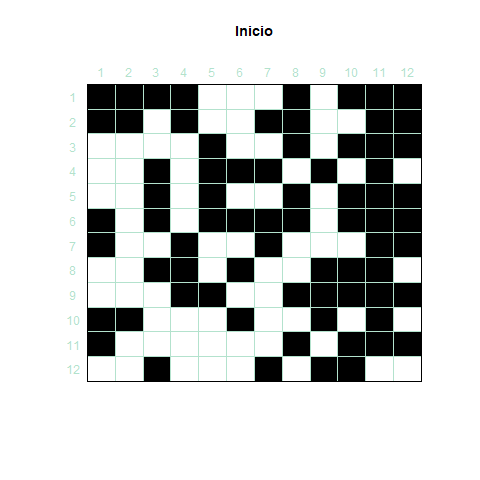
\includegraphics[width=60mm]{practica2_t0_r.png}
      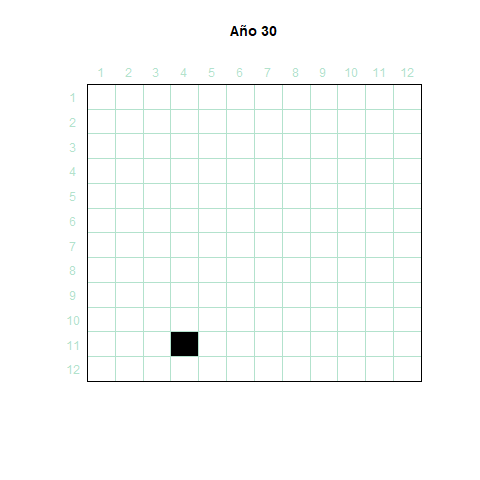
\includegraphics[width=60mm]{practica2_t30_r.png}
    \caption\\Secuencia de pasos de autómata celular{\label{Fig.1}
    \label{practica2_t0_r.png}}
\end{figure}

\justify De acuerdo a la interacción de pasos dados al cual llamaremos años se realizó un grafico que representa el numero de celdas vivas dependientes del paso de los años ver Fig. \ref{fig:my_label}
\begin{figure}[h]
    \centering
    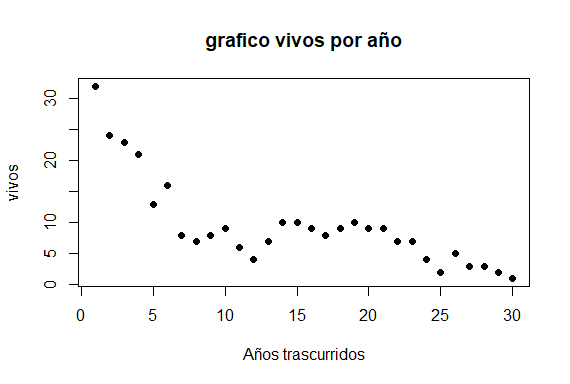
\includegraphics [width=70mm]{Rplot01.png}
    \caption   \\
    Grafico representativo de vivos en el trascurso de los 30 pasos {\label{fig}}
    \label{fig:my_label}
\end{figure}
\section{Conclusión}
 \justify Es de suma importancia comprender el diseño y ejecución de un experimento poniendo grados de complejidad, en este caso reglas de supervivencia con la finalidad de modelar un experimento de manera in situ antes de pasar al modo in vitro
\newpage
\bibliography{practica2} %\bibliography dentro de los corchetes aparece el comando seccion de referencias  sin embargo para que aparezca tiene que aparecer la seccion \bibliographystyle para dar un estilo del tipo de letra o tipo de acomodo que llevara 
\bibliographystyle{ieeetr}   %\da un estilo de acomodo dependiendo del comando dentro d corchetes
\end{document} %indica finalizacion de lo señalado en el parentesis en este caso el documento
